\documentclass[a4paper,twocolumn]{article}

% Učitaj pakete za kodnu stranicu 1250 i hrvatski jezik.
\usepackage[utf8]{inputenc}
\RequirePackage[croatian]{babel}

% Paket za hrvatski jezik neispravno izostavlja točke iza naslova,
% to ispravljamo zadavanjem novih funkcija za numeriranje koje stavljaju
% točku.
\makeatletter
\renewcommand\thesection{\@arabic\c@section.}
\renewcommand\thesubsection{\thesection\@arabic\c@subsection.}
\renewcommand\thesubsubsection{\thesubsection\@arabic\c@subsubsection.}
\renewcommand\theequation{\@arabic\c@equation}
\renewcommand\thefigure{\@arabic\c@figure.}
\renewcommand\thetable{\@arabic\c@table.}
\makeatother

% Ostali korisni paketi.
\RequirePackage{graphicx}
\RequirePackage{hyperref}
\RequirePackage{amssymb}
\RequirePackage{amsmath}
%\usepackage{mathrsfs}
\usepackage{listings}
\usepackage{algorithm}
\usepackage[noend]{algpseudocode}

\providecommand{\abs}[1]{\lvert#1\rvert}
\providecommand{\norm}[1]{\lVert#1\rVert}

% Ovdje započinje članak.
\begin{document}

% Navedite naslov i autore. Datume se automatski postavlja na datum kreiranja dokumenta,
% no može se promijeniti zadavanjem \date{30. veljače, 2004.}
\title{Detekcija pomaka u ugradbenim računalnim sustavima niske potrošnje}
\author{Josip Grlica, Ivan Pavić, Josip Puškar, Ivan Soldo, Ivan Spasić}
\maketitle

% Svako poglavlje započinje sa \section{Ime poglavlja} ako želimo da bude numerirano,
% a sa \section*{Ime poglavlja} ako ne želimo da bude numerirano.

\section*{Sažetak}
Rad daje pregled algoritama za detekciju pomaka. Detaljnije je obrađen princip
\(\Sigma\Delta\) estimacije pozadine. Algoritmi su stavljeni u kontekst implementacije u
ugradbenim računalnim sustavima niske potrošnje. Cilj rada je naći algoritam
za što robusniju detekciju uz očuvanje učinkovitosti. Algoritam koji je
implementiran jezgra je minimalnog sustava za videonadzor na \textit{BeagleBone
Black} platformi.

\section{Uvod}
Algoritam za detekciju pomaka mora precizno odvojiti objekte koji se kreću od
statične pozadine. Problem detekcije svodi se na klasifikaciju piksela slike
u dva razreda. Prvi razred je pozadina(engl. \textit{background}) kojoj odgovaraju
pikseli koji pripadaju statičnoj okolini. U drugi razred spadaju pomični
pikseli koji čine objekt koji se kreće(engl. \textit{foreground}). Pri klasifikaciji
piksela različiti su zahtjevi na osjetljivost i specifičnost detektora.
U tom smislu najvažnija je robustnost algoritma, odnosno prilagođenost pomičnim
objektima različitih brzina i veličina.

Zbog što veće autonomnosti sustava u pogledu napajanja,
sustav ne smije trošiti puno energije. Nadalje, prilikom obrade slike radi se s
relativno velikom količinom podataka što je memorijski i procesorski zahtjevno.
U radu osim pregleda metoda koje se već duže vrijeme koriste za estimaciju
pozadine razrađen je i način koji bi omogućio robusniju detekciju uz manju
potrošnju memorije i procesorske moći računala uz istovremeno smanjenje
potrošnje. Algoritam koji je razvijen temeljen je na principu \(\Sigma\Delta\)
estimacije koja se koristi u većini današnjih analogno digitalnih pretvornika.

\section{Metode estimacije pozadine slike}
Postoje razni načini estimacije pozadine slike. U ovom radu metode su
podijeljene u dvije skupine. Prilikom pregleda koristit će se sljedeće oznake:
\textit{I(t)} - slika u trenutku \textit{t}, \textit{B(t)} - pozadina u trenutku
\textit{t}.

\subsection{Metode diferenciranja}
Najjednostavnija metoda je oduzimanje okvira(engl. \textit{frame differencing}).
Metoda pretpostavlja da je pozadina u nekom trenutku \textit{t} jednaka slici
na ulazu. Metoda oduzima vrijednosti slike i pozadine na mjestu (\textit{x,y})
te apsolutnu vrijednost razlike uspoređuje s pragom odlučivanja. Zapisano
formulom za svaki pojedini piksel:
\begin{equation}
\abs{B(x, y, t) = I(x, y, t - 1)}
\end{equation}
\begin{equation}
\abs{I(x, y, t) - B(x, y, t)} > Th
\end{equation}
Konačno iz (1) i (2):
\begin{equation}
\abs{I(x, y, t) - I(x, y, t - 1)} > Th
\end{equation}

Nešto složenija metoda estimacije pozadine je procjena usrednjavanjem (engl.
\textit{mean filter}). Pretpostavka metode je da je pozadina u trenutku
\textit{t} jednaka usrednjenoj vrijednosti prethodnih slika u algoritam.

\begin{equation}
B(x, y, t) = \frac{1}{n}\sum\limits_{i=0}^{n-1}I(x, y, t - i)
\end{equation}
Za usporedbu s pragom koristimo izraz:
\begin{equation}
\abs{I(x, y, t) - \frac{1}{n}\sum\limits_{i=0}^{n-1}I(x, y, t - i)} > Th
\end{equation}

Mogu se koristiti i nelinearne metode. Primjer takve metode je procjena
medianom.

\begin{equation}
B(x, y, t) = median{(I(x, y, t - i))}
\end{equation}
\begin{equation}
\abs{I(x, y, t) - median{(I(x, y, t - i))}} > Th
\end{equation}
\begin{equation*}
i = 1,2..n
\end{equation*}

Velika prednost ovih metoda je što su jednostavne za implementaciju i
korištenje. Mogu biti relativno brze ako se implementiraju na pravilan način.
Srednja vrijednost pozadine nije konstantna i mijenja se s vremenom što ih
čini prilagodljivima na promjenu pozadine.

Nedostatak \textit{frame differencing} metode je to što preciznost ovisi o
brzini kretanja objekta na slici i vremena uzimanja pojedine slike
(engl. \textit{frame rate}). Nedostaci median metode i usrednjavanja su
memorijski i procesorski. Kod median metode ne može se odrediti median piksela
ako u memoriji ne postoji \textit{n} prethodnih piksela što zahtijeva veliki
potrošak memorije. U slučaju usrednjavanja potrošnja memorije može se izbjeći
metodom \textit{running average} ako prilagodimo izraz (4):
\begin{equation}
B(x, y, t) = \frac{t - 1}{t}B(x, y, t - 1) + \frac{1}{t}I(x, y, t)
\end{equation}
Međutim i ovakav pristup ima kritičan nedostatak. Naime ako je \textit{t} jako
velik ovo je teško numerički izvedivo na uređajima sa \textit{fixed-point}
aritmetikom. Još jedan nedostatak ovakvih metoda je fiksni globalni prag
za sve piksele koji nije promjenjiv s vremenom.

\subsection{Prilagodljivi modeli pozadine za praćenje u stvarnom vremenu}
U ovom poglavlju opisana je osnovna ideja modela pozadine
\textit{Adaptive Gaussian Mixture Model for Background Subtraction} prema
\cite{gaussian} dalje u tekstu GMM metoda (engl. \textit{Gaussian Mixture Model}).
GMM metoda je adaptivna metoda koja ima mogućnost prilagodbe multimodalnoj
pozadini. Koristi različiti prag odluke za svaki od piksela i dodatno je
taj prag promjenjiv u vremenu što rezultira dobrom prilagodbom na promjenu
osvjetljenja. Ipak, ako su promjene osvjetljenja nagle algoritam neće dobro
reagirati.

Algoritam na temelju početno izabranih parametara i početne pozadine generira
\textit{K} Gaussovih distribucija za pojedini piksel. Vrijednost parametra
\textit{K} je najčešće od 3 do 5, a svaka od distribucija osim varijance i
srednje vrijednosti sadrži parametar težine. Nadalje za svaki piksel u nekom
trenutku \textit{t} nalazi se optimalna od \textit{K} distribucija za piksel
odnosno provjerava se za koju distribuciju piksel upada unutar 2.5 standardne
devijacije distribucija. Ako se pronađe takva distribucija njezini parametri
se podešavaju na sljedeći način:
\begin{equation*}
\mu_{(x,y), t} = (1 - \rho)\mu_{(x,y), t - 1} + \rho I(x,y,t)
\end{equation*}
\begin{equation*}
\sigma^{2}_{(x,y), t} = (1 - \rho)\sigma^{2}_{(x,y), t-1} + \rho(I(x,y,t) -
\sigma^{2}_{(x,y), t-1})^2
\end{equation*}, gdje je:
\begin{equation*}
\rho = \alpha N(I(x,y,t)|\mu_{(x,y), t-1},\sigma^{2}_{(x,y), t-1})
\end{equation*}
a \(\alpha \) je \textit{learning rate}. Nakon podešavanja parametara razdiobe
podešavaju se i težine razdioba:
\begin{equation*}
\omega_{(x,y), t} = (1 - \alpha)\omega_{(x,y), t-1} + \alpha M_{(x,y), t}
\end{equation*}
gdje je \(M_{(x,y), t} = 1\) za pronađenu distribuciju \(M_{(x,y), t} = 0\) za
ostale distribucije. Ako odgovarajuća distribucija nije pronađena koriste se
različite heuristike za generiranje novih distrubicija. Jedan od kriterija je
i \(\omega/\sigma\) kriterij. Nove generirane distribucije imaju veliku
varijancu i malu težinu.

\section{Metoda procjene pozadine \(\Sigma\Delta\) algoritmom}

\(\Sigma\Delta\) procjena pozadine je jednostavna nelinearna metoda oduzimanja
pozadine (engl. \textit{background subtraction}) zasnovana na usporedbi i
jediničnom inkrementu. U nastavku ovog poglavlja razrađeni su principi metode
i dani su primjeri algoritama. Dodatno, algoritam je uspoređen s ostalim
algoritmima za procjenu pozadine.

\subsection{Rekurzivne procjene pozadine}

Uz pretpostavku da je svaki piksel slike na ulazu u algoritam opisan nekom
funkcijom \(f_i(t)\) najjednostavniji način procjene vrijednosti pojedinog
piksela bilo bi naći srednju vrijednost \(f_i(t)\). Takav pristup je već
razrađen i predstavljen je izrazom (8). Općenito se srednja vrijednost signala
u trenutku \(t\) može prikazati izrazom (u nastavku zbog jednostavnijeg zapisa
promatra se samo vremenska dimenzija signala):
\begin{equation}
M_t = \frac{1}{t}I_t + \frac{t-1}{t} M_{t-1}
\end{equation}
Ovakav pristup je numerički neizvediv za duže nizove stoga se uvodi konstantna
težina (\(\alpha\)) i dobiva generički zapis:
\begin{equation}
M_t = \alpha I_t + (1 - \alpha)M_{t-1}
\end{equation}
Ova jednadžba predstavlja \textit{running average} metodu. Rješavanjem
rekurzivne jednadžbe u \(Z\) domeni, očito je da se radi o niskopropusnom
filtru (tzv. \textit{exponential smoothing} filter).
Posljednji izraz može se  prikazati u inkrementalnom obliku
\begin{equation}
M_t = M_{t-1} + \delta_t(I_t)
\end{equation}
Ovisno o trenutnom uzorku signala mijenja se srednja vrijednost. U osnovnom
slučaju \(\delta_t(I_t) = \alpha(I_t - M_{t-1})\) funkcija inkrementa je linearna
i što je veća razlika \(\Delta\) između trenutnog uzorka signala i pozadine veći
je utjecaj na procjenu pozadine što u osnovi nije dobro jer će male promjene
biti u potpunosti zanemarene. Stoga se uvode različite težine \(\alpha\) za
različiti raspon \(\Delta\). Najčešće se uzima veća težina za one područja
koja se smatraju pozadinom. Za dvije različite težine stoga se uzima jedan
fiksni prag. Postavljanje fiksnog praga je kritično u ovakvom načinu procjene
radi diskontinuiteta.

\begin{figure}[htb]
\begin{center}
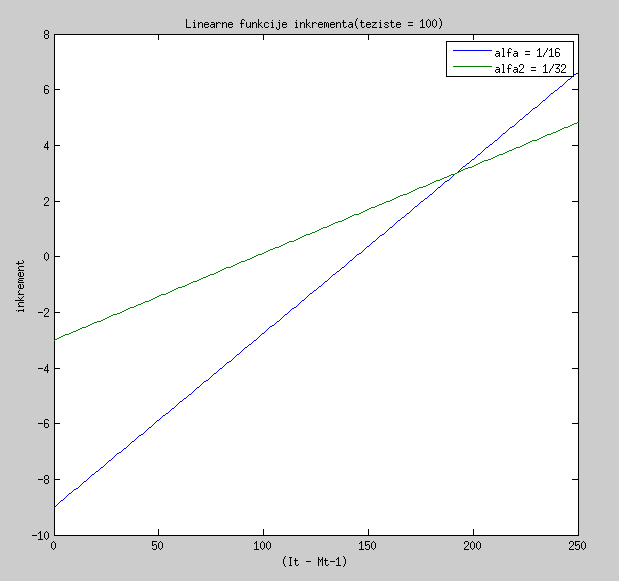
\includegraphics[height=5cm]{afina1.png}
\caption{Linearna funkcija inkrementa}
\end{center}
\end{figure}

\begin{figure}[htb]
\begin{center}
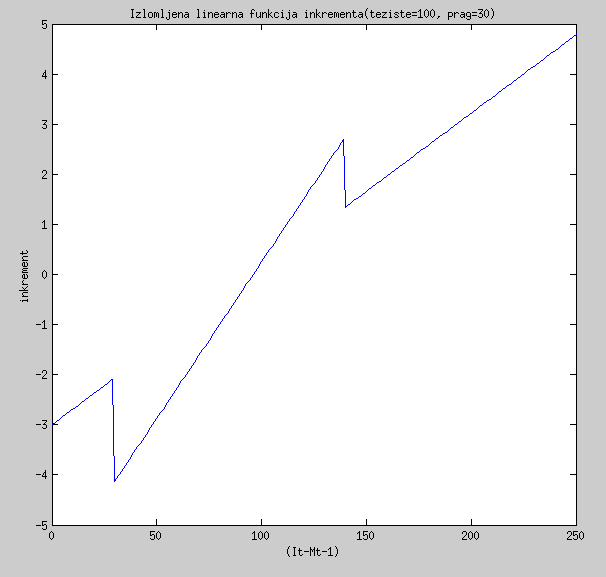
\includegraphics[height=5cm]{afina2.png}
\caption{Izlomljena linearna funkcija inkrementa}
\end{center}
\end{figure}

Osim inkrementa oblika linearne funkcije \cite{zipf} predlaže koristiti i
inkrement oblikovan Gaussovom distribucijom. Ipak, u daljnjem razmatranju neće
se koristiti.

\begin{equation}
\delta_t = \alpha_{max} e^{\frac{-(I_t - M_{t-1})^2}{2V_{t-1}}}(I_t - M_{t-1})
\end{equation}

\begin{figure}[htb]
\begin{center}
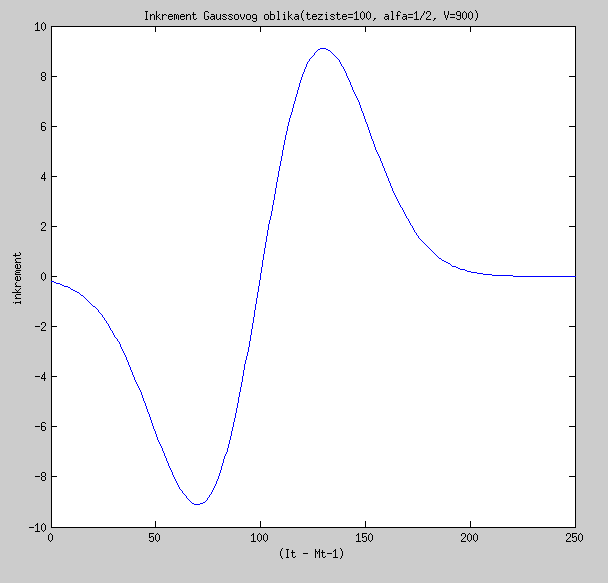
\includegraphics[height=5cm]{gauss.png}
\caption{Funkcija inkrementa Gaussovog oblika}
\end{center}
\end{figure}


\subsection{Zipfova razdioba i procjena pozadine}

U daljnim razmatranjima koristit će se Zipfova distribucija za oblikovanje
funkcije inkrementa. Zipfova distribucija odnosno Zipfov zakon izvorno je
empirijski pokazan. Najpoznatiji primjer iz teorije informacije i lingvistike
je pojava da je vjerojatnost pojave \textit{n-te} najčešče riječi \(1/n\).
Općenito, radi se o Zipf-Mandelbrot razdiobi čija je se funkcija razdiobe
prema \cite{zipf} može napisati:
\begin{equation}
Z_{(\mu, k, s)}(x) = \frac{(s-1)k^{s-1}}{2(\abs{x - \mu} + k)^s}
\end{equation}
gdje je \(\mu\) težište razdiobe, \(k\) varijanca. Ako iskoristimo ovakvu
funkciju distribucije za oblikovanje inkrementa, tada inkrement postaje
funkcija nalik step funkciji odnosno \(\delta_t = \kappa\) za \(x > 0\)
\(\delta_t = -\kappa\) za \(x < 0\) pri čemu je \(\kappa = \alpha * k^s\).
Ovo ponašanje direktno vodi na vezu između procjene srednje vrijednosti signala
jediničnim inkrementom u \(\Sigma\Delta\) analogno digitalnim pretvornicima i
Zipfove distribucije. Dodatno, određen je statistički model za promatranu
pozadinu pa u samoj estimaciji koriste pretpostavljena statistička
svojstva modela.

\begin{figure}[htb]
\begin{center}
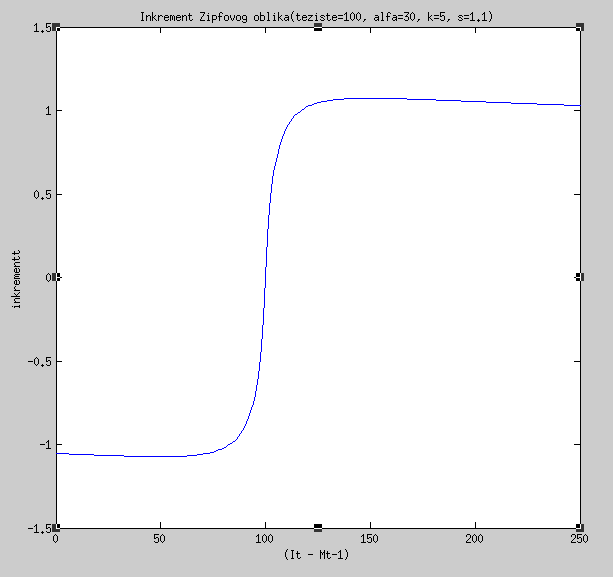
\includegraphics[height=5cm]{zipf.png}
\caption{Funkcija inkrementa Zipfovog oblika}
\end{center}
\end{figure}

\subsection{Osnovni \(\Sigma\Delta\) algoritam}

Osnovni princip \(\Sigma\Delta\) algoritma je procijeniti parametre pozadine koristeći
\(\Sigma\Delta\) modulaciju što je tipično u analogno digitalnoj pretvorbi. Za signal
promjenjiv u vremenu \(f_t\) procjenjuje se diskretni signal \(d_t\) uzorkovan
određenom frekvencijom. Za procjenu svakog uzorka diskretnog signala \(i\)
koriste sljedeći izrazi:
\begin{equation}
d_t(i) = d_t(i-1) - \epsilon
\end{equation}
za \(d_t(i-1) < f_t(i)\), odnosno:
\begin{equation}
d_t(i) = d_t(i-1) + \epsilon
\end{equation}
za \(d_t(i-1) > f_t(i)\) pri čemu je \(\epsilon\) korak diskretizacije.

U \(\Sigma\Delta\) računanju pozadine, ulazni signal je vrijednost svakog
piksela u vremenu \(I_t\), iz kojeg se proračunava težinski estimator pozadine
\(M_t\). Zatim se računa apsolutna razlika između vrijednosti piksela ulaznog
signala \(I_t\) i težinskog estimatora pozadine \(M_t\). Na temelju toga se izračunava
estimator varijance \(V_t\). Parametar za estimaciju varijance
je \(N\) čija je tipična vrijednost između 1 i 4.


\makeatletter
\def\BState{\State\hskip-\ALG@thistlm}
\makeatother

\begin{algorithm}
\caption{Osnovni \(\Sigma\Delta\) algoritam}\label{euclid}
\begin{algorithmic}[1]
\For{svaki piksel}
\If {\(M_{t-1}(x) < I_t(x)\)}
  \State{\(M_{t}(x) = M_{t-1}(x) + 1\)}
\ElsIf {\(M_{t-1}(x) > I_t(x)\)}
  \State{\(M_{t}(x) = M_{t-1}(x) - 1\)}
\Else
  \State{\(M_{t}(x) = M_{t-1}(x)\)}
\EndIf
\EndFor
\For{svaki piksel}
  \State{\(O_{t}(x) = \abs{M_{t}(x) - I_t(x)}\)}
\EndFor
\For{svaki piksel}
\If {\(V_{t-1}(x) < N * O_t(x)\)}
  \State{\(V_{t}(x) = V_{t-1}(x) + 1\)}
\ElsIf {\(V_{t-1}(x) > N * O_t(x)\)}
  \State{\(V_{t}(x) = V_{t-1}(x) - 1\)}
\Else
  \State{\(V_{t}(x) = V_{t-1}(x)\)}
\EndIf
\EndFor
\For{svaki piksel}
\If {\(O_{t}(x) < V_t(x)\)}
  \State{\(E_{t}(x) = 0\)}
\Else
  \State{\(E_{t}(x) = 1\)}
\EndIf
\EndFor
\end{algorithmic}
\end{algorithm}

\subsection{\(\Sigma\Delta\) algoritam s uvjetnim inkrementom}
U osnovnoj inačici algoritma nisu se koristila statistička svojstva modela.
\cite{sigma} predlaže da se ona mogu koristiti i da impliciraju sljedeća
svojstva. Frekvencija osvježavanja pozadine proporcionalna je varijanci
razdiobe, a varijanca se osvježava s nekim konstantnim periodom \(Tv\).
Prilagođeni algoritam vrlo je sličan početnom algoritmu, a \cite{zipf} predlaže
da se algoritam izvede ovako:
\begin{algorithm}
\caption{Zipf \(\Sigma\Delta\) algoritam}\label{zipf}
\begin{algorithmic}[1]
\For{svaki trenutak t}
\State{\(rank = t \% 2^m;\)}
\State{do \{pow2 = 2 * pow2\}}
\State{while((\(rank \% 2 == 0\)) and (\(pow2 < 2^m\)))}
\If {\(V_{t-1}(x) > 2^m/pow2\)}
  \State{estimiraj pozadinu za svaki piksel}
\EndIf
\State{\(O_{t}(x) = \abs{M_{t}(x) - I_t(x)}\)}
\If {\(t \% Tv == 0\)}
  \State{estimiraj varijancu za svaki piksel}
\EndIf
\EndFor
\end{algorithmic}
\end{algorithm}

\subsection{Usporedba \(\Sigma\Delta\) algoritma s GMM algoritmom}
GMM algoritam zahtijeva računski puno više posla za svaki piksel (usporedbe
u kontekstu \textit{K} distribucija) dok se kod \(\Sigma\Delta\) algoritma radi
o uvjetnom jediničnom inkrementu. Memorijski je zahtjevnije jer je za svaki
piksel moraju pamtiti \textit{K} srednjih vrijednosti, varijanci i težina i
najčešće je potrebno raditi operacije nepogodne za \textit{fixed-point}
aritmetiku. Kod \(\Sigma\Delta\) algoritma sve operacije su jednostavnije
(usporedba, inkrement, apsolutna razlika) i manja je potrošnja memorije
(pamti se matrica estimatora pozadine i varijance).

\subsection{Analiza implementacije \(\Sigma\Delta\) algoritma}
Osnovni \(\Sigma\Delta\) algoritam neće dati dobre rezultate u svim situacijama.
Osim toga ovisno o periodu osvježavanja težinskog estimatora \(M_t\) dobivaju
se različiti rezultati. Uz pomno odabranu konstantu \(N\) za varijancu može
se ukloniti velik dio šuma. Ipak za bolje rezultate poželjno je koristiti i
neko od morfoloških filtriranja za dodatno uklanjanje šuma. U nastavku su
prikazane rezultati evaluacije algoritma u pokaznoj situaciji:

\begin{figure}[bp!]
\begin{center}
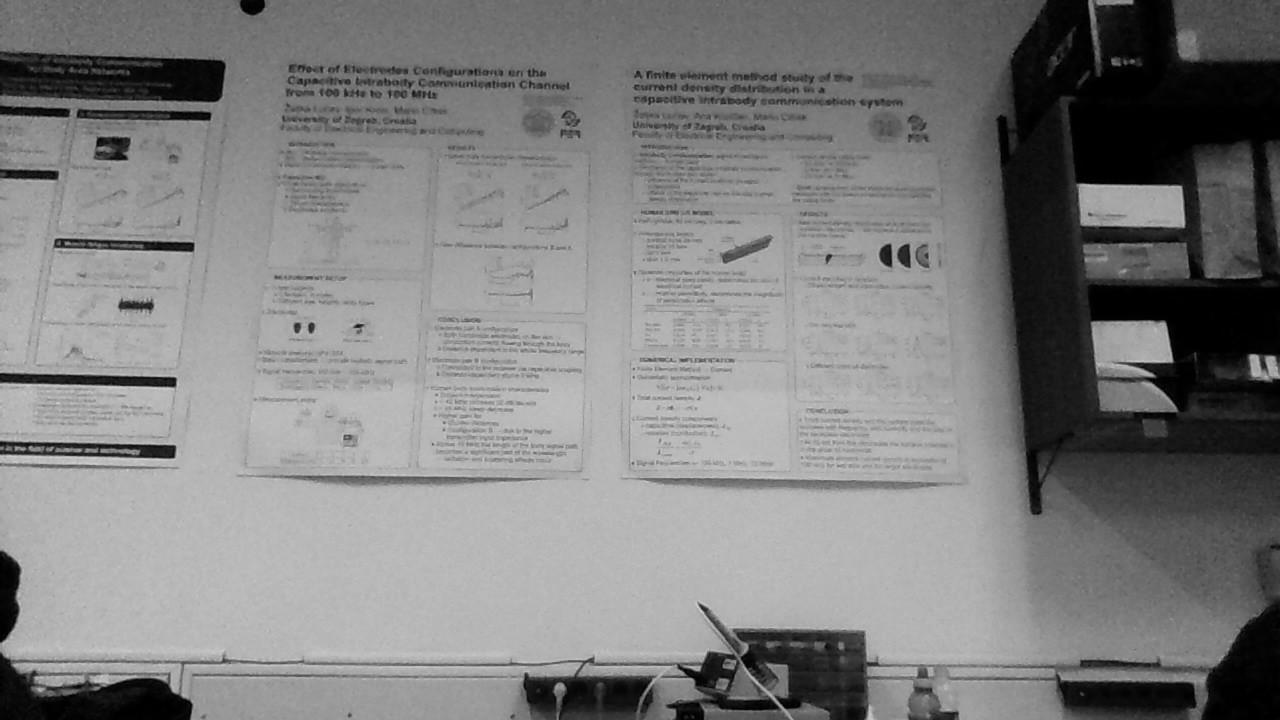
\includegraphics[width=5cm]{background.jpg}
\caption{Slika pozadine}
\end{center}
\end{figure}
\begin{figure}[bp!]
\begin{center}
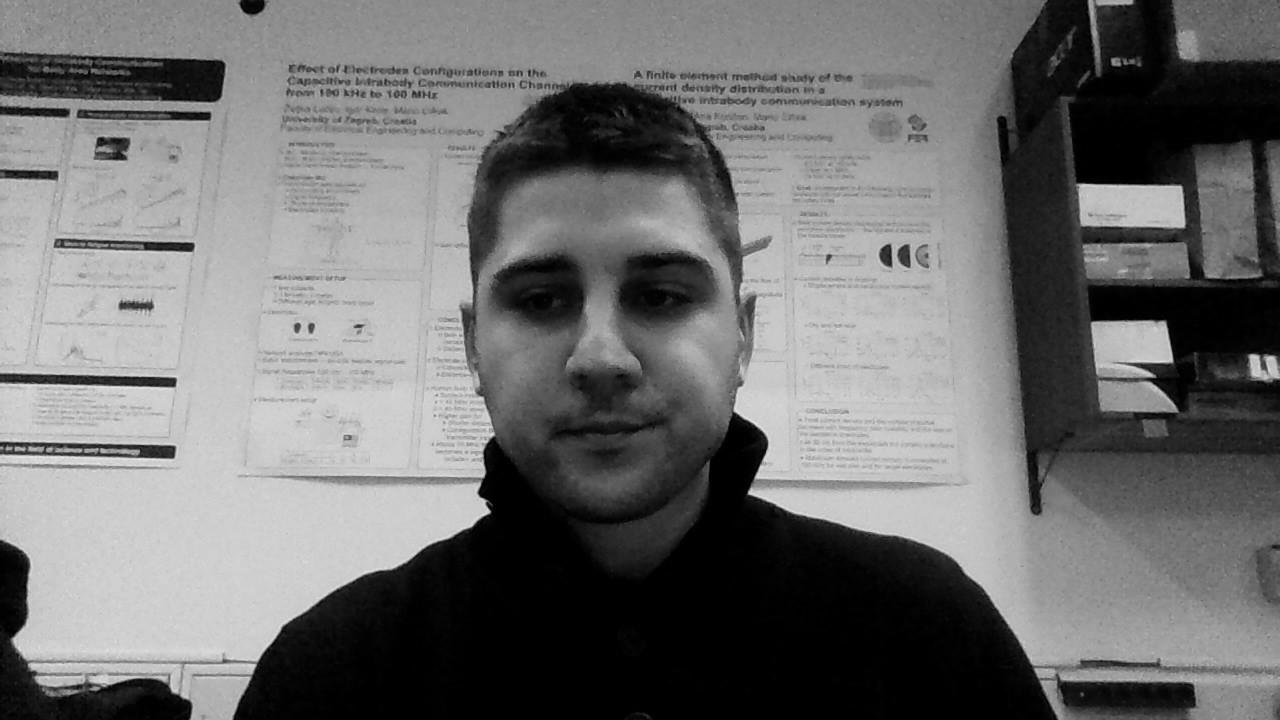
\includegraphics[width=5cm]{foreground.jpg}
\caption{Slika pomaka}
\end{center}
\end{figure}
\begin{figure}[bp!]
\begin{center}
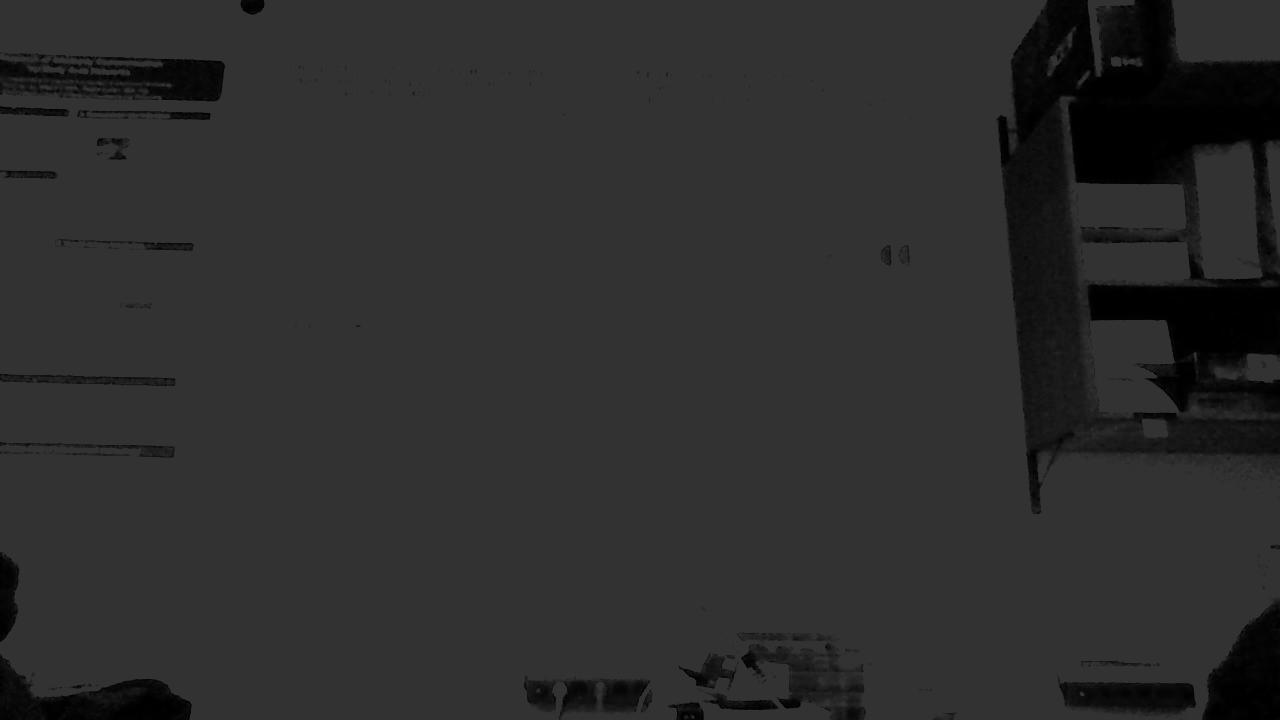
\includegraphics[width=5cm]{modeEstimation.jpg}
\caption{Estimacija srednje vrijednosti \(M_t\) - 50 koraka algoritma}
\end{center}
\end{figure}
\begin{figure}[bp!]
\begin{center}
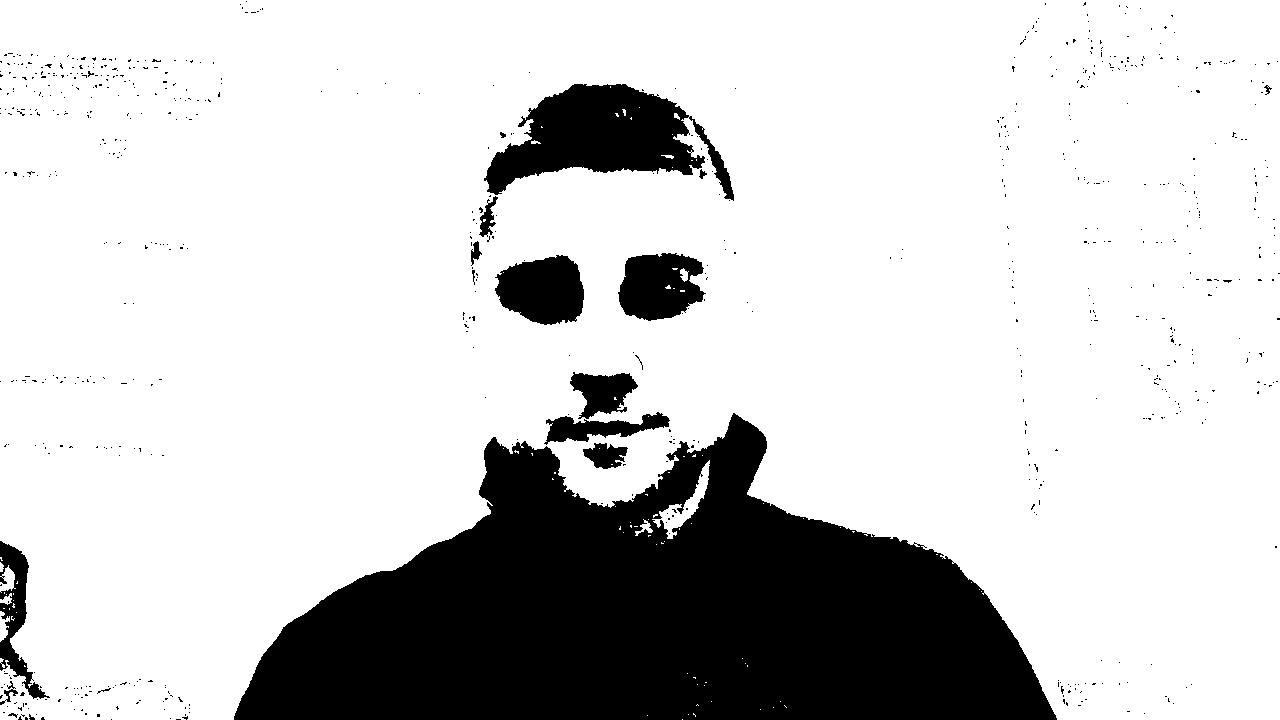
\includegraphics[width=5cm]{sigmadeltamask.jpg}
\caption{Maska nakon jednog koraka algoritma \(M_t\)}
\end{center}
\end{figure}


\section{Sustav za videonadzor}
Uz pomoć razvijenog algoritma napravljen je jednostavan sustav za videonadzor
temeljen na \textit{BeagleBone Black} platformi. Idejna shema sustava prikazana
je na slici \ref{fig:sustav}.
\begin{figure}[bp!]\label{sustav}
\begin{center}
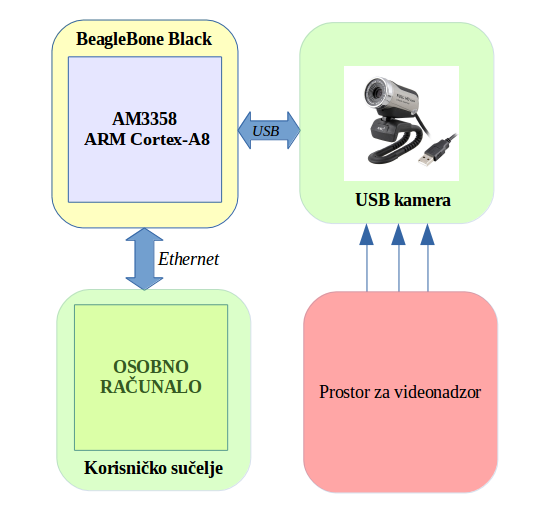
\includegraphics[height=5cm]{sustav_shema.png}
\caption{Razvijeni sustav za videonadzor}
\end{center}
\label{fig:sustav}
\end{figure}

\textit{BeagleBone Black} platforma prikuplja podatke sa kamere. Podaci se
zatim obrađuju \(\Sigma\Delta\) algoritmom, a na temelju čeka se daljnom
analizom binarne maske koja se dobije na izlazu \(\Sigma\Delta\) algoritma
utvrđuje da li je došlo do pomaka ili ne. Korisnik je preko interaktivnog
sučelja dostupnog u lokalnoj mreži obaviješten o eventualnom detektiranom
pomaku. Nadalje korisniku je preko korisničkog sučelja dostupan pregled slika
svih detektiranih pomaka, a svaki detektirani pomak spremljen je u bazu
podataka s pripadajućim vremenom i datumom detekcije. Korisničko sučelje ima
zvučni i vizualni alarm u slučaju detektiranog pomaka. Putem korisničkog sučelja
korisnik može podešavati parametre algoritma za detekciju pomaka.

\subsection{Analiza programske podrške}
Programska podrška sastoji se od 2 procesa. Jedan od procesa zadužen je
za akviziciju i obradu slike prema zadanim parametrima. Drugi proces je
poslužitelj koji korisniku omogućava promjenu parametara algoritama za obradu
slike. Poslužitelj generira sučelje i sadržava stanje sustava za detekciju
pomaka. Sustav može biti u jednom od 3 stanja. Prvo stanje je inicijalno u koje
sustav dolazi nakon pokretanja i traje određeno vrijeme koje je potrebno sustavu
da procjeni pozadinu i započne s normalnim radom. Iz početnog stanja sustava
sustav prelazi u drugo stanje u kojem nema pomaka. U trećem stanju sustav je
detektirao pomak. Ovisno o stanju sustava, sustav sprema podatke o okolini.
Konkretno, spremanje slika u memoriju moguće je samo iz stanja u kojem je
pomak detektiran. Poslužitelj je stoga odgovoran i za spremanje slika u bazu
podataka. Između poslužitelja i procesa za obradu slike postoji međuprocesna
komunikacija putem \textit{Unix domain socket} protokola. Na taj način je
prije svega omogućeno prosljeđivanje slike iz procesa za obradu slike do
krajnjeg korisnika (engl. \textit{stream}). Osim prijenosa slike prenosi se
i informacija o detekciji pomaka, odnosno je li pomak detektiran ili nije.
Na isti način poslužitelj ovisno o parametrima koje mijenja korisnik na sučelju
šalje parametre procesu za obradu slike koji te iste parametre prilagođava.

Za razvoj programske podrške za obradu slike korištena je programska biblioteka
\textit{OpenCV 3.1}. Za razvoj programske podrške za server korišten je
\textit{Node.js framework}.

\begin{figure}[hp!]
\begin{center}
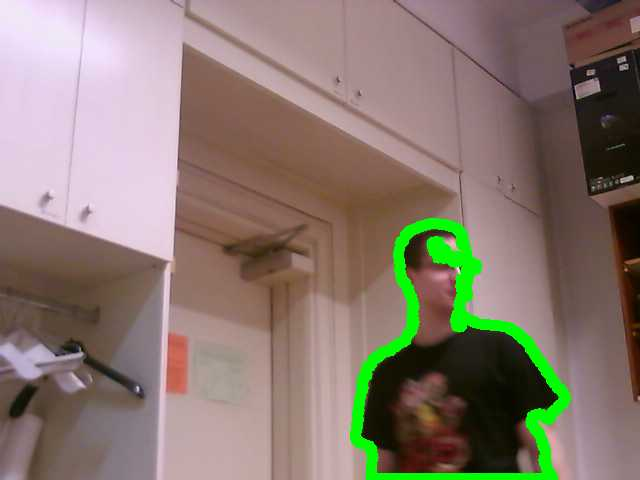
\includegraphics[height=5cm]{interface.jpeg}
\caption{Prikaz konačnog rezultata obrade dostupnog na web sučelju}
\end{center}
\end{figure}




\section{Zaključak}

Detekcija pomaka i analiza pozadine slike jedna je od ključnih tema u računalnom
vidu. Postoji mnogo metoda, a samo su neke razrađene u ovom radu. Pokazano je
kako su operacije nad slikama procesorski i memorijski zahtjevne i zbog toga se
traže novi načini i metode obrade. Jedan od njih je \(\Sigma\Delta\) pristup
estimaciji pozadine. Najvažnije prednosti \(\Sigma\Delta\) pristupa u odnosu
na ostale pristupe je jednostavnost računskih operacija. Potrebne su svega
tri operacije za provedbu algoritma: apsoultna razlika, usporedba i inkrement
odnosno dekrement. Jednostavnost operacija omogućava i sklopovsku realizaciju
algoritma koja može dodatno ubrzati proces estimacije. Pošto je estimacija
pozadine početni korak u daljnoj analizi slike kao što je primjerice predikcija
kretanja bitno je da se izvršava što brže radi zadovoljenja zahtjeva za obradu
u realnom vremenu. Stoga će slični modeli i principi u budućnosti biti sve
aktualniji.


% Literatura se automatski generira iz zadane liste. Svaki od elemenata liste
% započinje s oznakom, npr. \bibitem{davies}. U tekstu se referenca na članak
% ili knjigu dobiva s \cite{davies}.
\begin{thebibliography}{25}

\bibitem{sigma}
Lacassagne, L. ; IEF/AXIS, Univ. Paris Sud, Paris, France ; Manzanera, A. ;
Dupret, A.
Motion detection: Fast and robust algorithms for embedded systems

\bibitem{zipf}
A.~Manzanera ENSTA - Elec. and Comp. Sc. lab, 32 Bd Victor, 75015 Paris, France
\(\Sigma-\Delta\) background subtraction and the Zipf law

\bibitem{gaussian}
Z.~Zivkovic,
Improved Adaptive Gaussian Mixture Model for Background Subtraction

\bibitem{simple}
B.~Tamersoy,
Background Subtraction
http://www.cs.utexas.edu

\end{thebibliography}

\end{document}
